\documentclass{zjgsureport}

% ---------------------虚线部分需填入个人信息---------------------
% 封面的题目,请修改
\mytitle{课程论文模板}
% 封面的课程名称,请修改
\course{课程名}
% 封面的学院,请修改
\college{学院名}
% 封面的专业,请修改
\major{专业名}
% 封面的班级,请修改
\class{班级名}
% 封面的学号,请修改
\stuid{你的学号}
% 封面的学生姓名,请修改
\name{你的名字}
% 封面的成绩,留白,无需修改
\score{  }
% 封面的日期,无需修改
\date{\today}
% ---------------------虚线部分需填入个人信息---------------------

% 重定义摘要二字的大小
\renewcommand{\abstractname}{\large \heiti \bfseries 摘要\\}
% 更改section的自动编号方式、字体,并设置为四号字体
\titleformat*{\section}{\large\heiti\bfseries}
\renewcommand\thesection{\zhnum{section}、}
% 更改网址url字体为空,即跟随主文字字体
\def\UrlFont{}
% 设置图片表格为五号,粗体
\captionsetup{font={small,bf},labelsep=quad}
% 更改subsection的自动编号方式并设置字体大小
\titleformat*{\subsection}{\normalsize\heiti\bfseries}
\titleformat*{\subsubsection}{\normalsize\heiti\bfseries}
\renewcommand\thesubsection{\arabic{section}.\arabic{subsection}}
% 更改公式自动编号的方式,并做到每重开一章,重新计数
\makeatletter
\@addtoreset{equation}{section}
\makeatother
\renewcommand{\theequation}{\arabic{section}.\arabic{equation}}
% 改动参考文献标题的字体大小为四号
\renewcommand{\refname}{\large \heiti \bfseries 参考文献}
% 引用时变上标
\newcommand{\upcite}[1]{\textsuperscript{\textsuperscript{\cite{#1}}}}
% 更改附录名
\renewcommand\appendix{\par
    \setcounter{section}{0}
    \setcounter{subsection}{0}
    \gdef\thesection{附录\zhnum{section}}}


% ----------------------下面是文章内容,请填入自己的文章----------------------
% ---------------------为方便修改每一章节,推荐使用input---------------------
\begin{document}
% 0. 使用新的日期格式
\DTMsetdatestyle{mydatestyle}
% 1. 生成封面
\makecover
% 2. 摘要
\thispagestyle{empty}
% 2.1 全文标题,请重新输入
\begin{center}
    {\heiti \myLarge 课程论文模板}
\end{center}
% 2.2 摘要内容
\begin{abstract}
请在这里输入摘要内容.

{\bfseries 关键词:关键词1,关键词2,关键词3}
\end{abstract}
\clearpage
% 3. 目录
\thispagestyle{empty}
\tableofcontents
\clearpage
% 4. 正文,并从这里开始生成页码
\setcounter{page}{1}
\section{你的一级标题}
\subsection{你的二级标题1}
在日常生活中,我们所拍摄的对象时常不会处于完全静止的状态,而由于其运动,所拍摄的照片会产生许多噪声。但是用一些简单的逆滤波方法不能很好地处理噪声需要采用约束复原的方法,维纳滤波(最小均方误差滤波器)复原就是一种有代表性的约束复原方法,是使原始图像$f(x,y)$和复原图像$\hat{f}(x,y)$之间均方误差最小的复原方法。

均方误差的表达式为:
\begin{equation}
    e^2=E\left[(f-\hat{f})^2\right]
\end{equation}

\subsection{你的二级标题2}
为方便理解,现将代码中部分用到的函数的作用放入下表做简单介绍:
    \begin{table}[H]
        \begin{center}
        \caption{对模糊加噪声图像进行维纳滤波复原代码中函数的介绍}
        \label{tab:codedes}
        \begin{tabular}{|c|c|}
            \hline
            函数 & 作用 \\ \hline
            {\ttfamily imread(filename.fmt)} & \tabincell{c}{根据文件名{\ttfamily filename}读取灰度获彩色图像,\\返回的是包含图像数据的数组}\\ \hline
            {\ttfamily rgb2gray(RGB)} & \tabincell{c}{消除图像色调和饱和度信息同时保留亮度\\将{\ttfamily RGB}图像或彩色图转换为灰度图像}\\ \hline
            {\ttfamily im2double(I)} & 将灰度图像{\ttfamily I}转换为双精度\\ \hline
            {\ttfamily size(A)} & 获取矩阵{\ttfamily \textit{A}}的行数和列数\\ \hline
            {\ttfamily fspecial(type, para)} & \tabincell{c}{用于建立预定义的滤波算子,\\其中{\ttfamily type}指定算子的类型,\\{\ttfamily para}指定相应的参数}\\ \hline
            {\ttfamily conv2(A,B)} & 计算矩阵{\ttfamily \textit{A}}和{\ttfamily \textit{B}}的卷积\\ \hline
            {\ttfamily zeros(m,n)} & 产生{\ttfamily \textit{m}}$\times${\ttfamily \textit{n}}的零矩阵\\ \hline
            {\ttfamily imnoise(f,type,parameters)} & \tabincell{c}{给一幅图像添加噪声,{\ttfamily f}是原图像,\\{\ttfamily type}是加入的噪声类型,\\{\ttfamily parameters}是噪声的一些参数}\\ \hline
            {\ttfamily figure} & 创建一个新的窗口,所有参数采用默认\\ \hline
            {\ttfamily imshow(I)} & 显示灰度图像{\ttfamily I}\\ \hline
            {\ttfamily title('caption')} & 设置图像的标题{\ttfamily caption}\\ \hline
        \end{tabular}
    \end{center}
    \end{table}

表格引用:表\ref{tab:codedes}.

\subsection{你的二级标题3}
代码运行结果如下:
    \begin{figure}[htbp]
        \centering
        \subfigure[加噪声的模糊图像]
        {
            \centering
            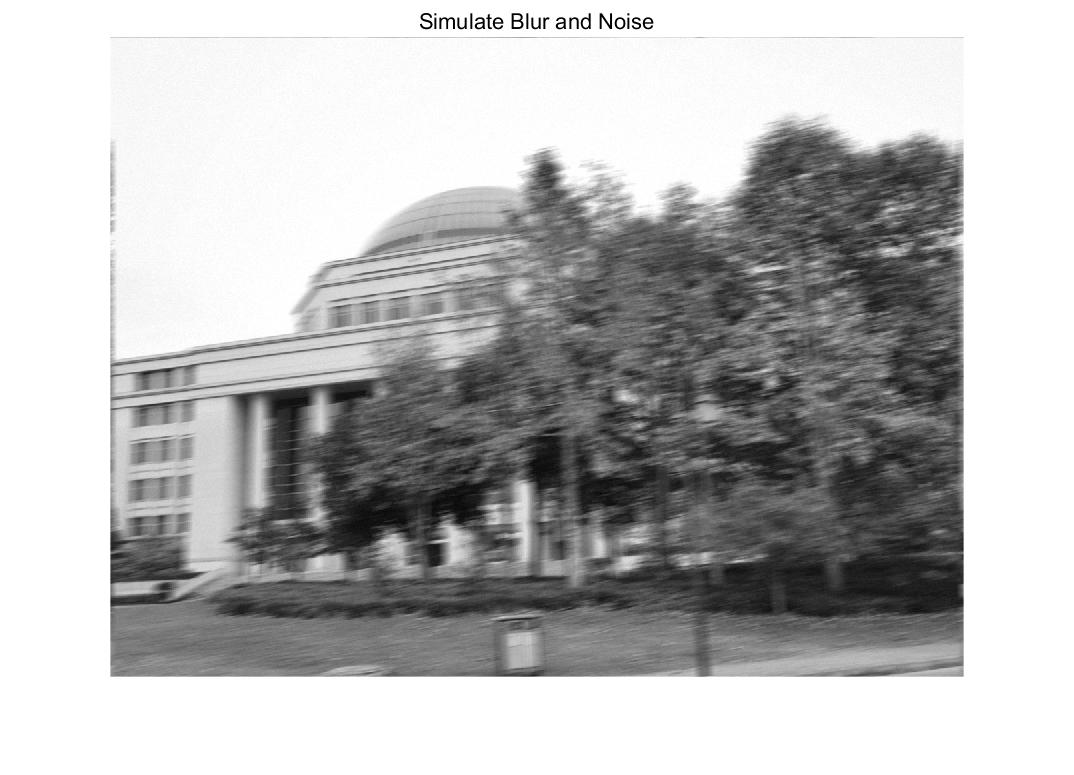
\includegraphics[scale=0.22]{images/pic2-2.2.2-1.jpg}
        }
        \subfigure[维纳滤波结果图像]
        {
            \centering
            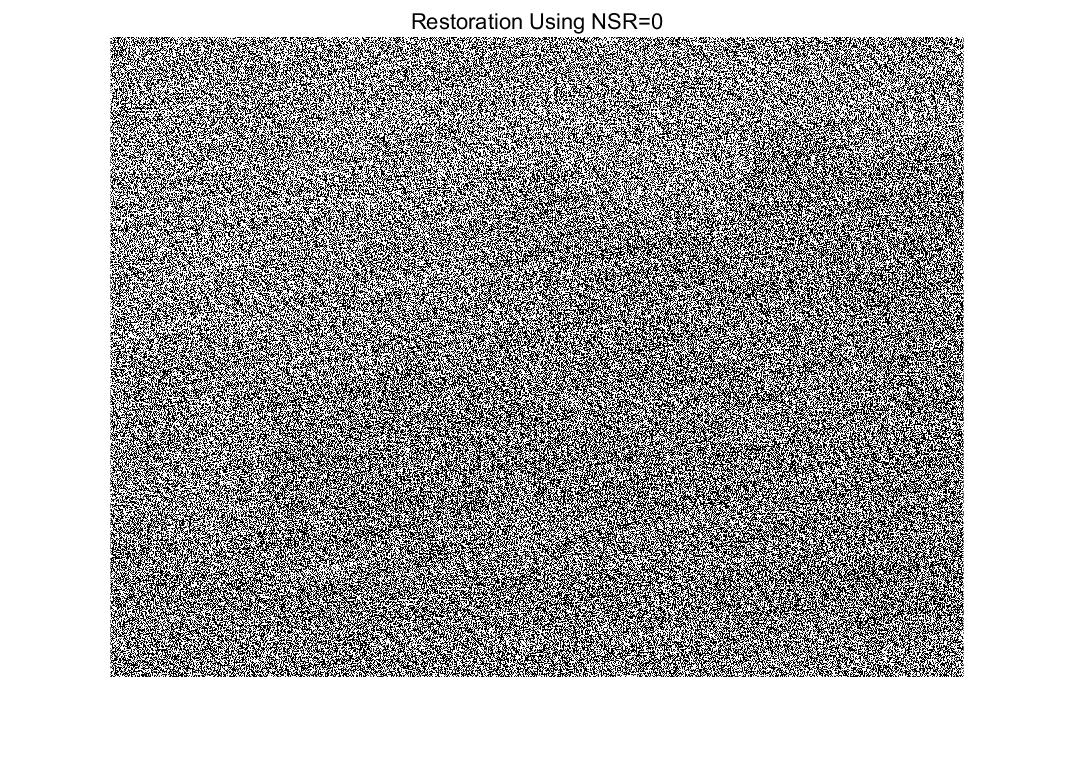
\includegraphics[scale=0.22]{images/pic2-2.2.2-2.jpg}
        }
        \caption{维纳滤波效果}
        \label{fig:result}
    \end{figure}

图片引用:图\ref{fig:result}.


\subsection{你的二级标题4} \label{else}

章节引用:节\ref{else}。

文献引用:\cite{cai}或\upcite{cai}。

Matlab代码参见\ref{app:1}.
\clearpage

% 5. 参考文献
\begin{thebibliography}{99}
    \bibitem{cai}蔡利梅,王利娟. 数字图像处理. 徐州:中国矿业大学出版社, 2014.08.
\end{thebibliography}
\clearpage

% 6. 附录
\appendix
\small
\section{Matlab代码} \label{app:1}
\begin{lstlisting}[language=matlab]
Image=im2double(rgb2gray(imread('pic2.jpg')));
window=15;
[n, m]=size(Image);
n=n+window-1;
m=m+window-1;
% 点扩散函数
h=fspecial('average', window);
BlurredI=conv2(h, Image);
% 噪声信号
noise=imnoise(zeros(n, m),'salt & pepper', 0.001);
% 给模糊图像添加椒盐噪声
BlurrednoisyI=BlurredI+noise;
figure, imshow(BlurrednoisyI), title('Blurred Image with noise');
% 模板延拓
h1=zeros(n, m);
h1(1:window, 1:window)=h;
H=fftshift(fft2(h1));
% 计算信噪比
K=sum(noise(:).^2)/sum(Image(:).^2);
% 计算维纳滤波传递函数
M=conj(H)./(abs(H).^2+K);
G=fftshift(fft2(BlurrednoisyI));
f=ifft2(ifftshift(G.*M));
result=f(1:n-window+1, 1:m-window+1);
figure, imshow(abs(result), []), title('Filtered Image');
\end{lstlisting}
\end{document}
% ---------------------上面是文章内容,请填入自己的文章---------------------